\documentclass[a4j, twocolumn]{jarticle}
\usepackage{graphicx}
\usepackage{titling}
\graphicspath{{./images/}}

\begin{document}
  \title{インドネシア \\\large 東南アジアの隠れた美しさ}
  \author{Christian Harjuno\thanks{釧路工業高等専門学校情報工学科}}
  \date{\today}
  \maketitle
  \section{インドネシアってなんですか?}
  インドネシア, またはインドネシア共和国は, 東南アジアにある国の一つです. 赤道の中央に位置し, インドネシアの列島はシンガポール, マレーシア, オーストラリアの間にあります. 2020年の国勢調査によると, インドネシアの人口は約2億7千万人で, 世界で4番目に多いです. 
  インドネシアについてよく知っている外国の方は少ないと思います. 「インドネシアについて何かご存知ですか」と聞けば, 最も多い答えは「バリ島」ですが, 実際のインドネシアはそれ以上にすばらしい国だと思います. したがって, 今回はインドネシアについてより詳しく説明したいと思います. 
  \section{地理と多様性}
  \begin{figure}
    \centering
    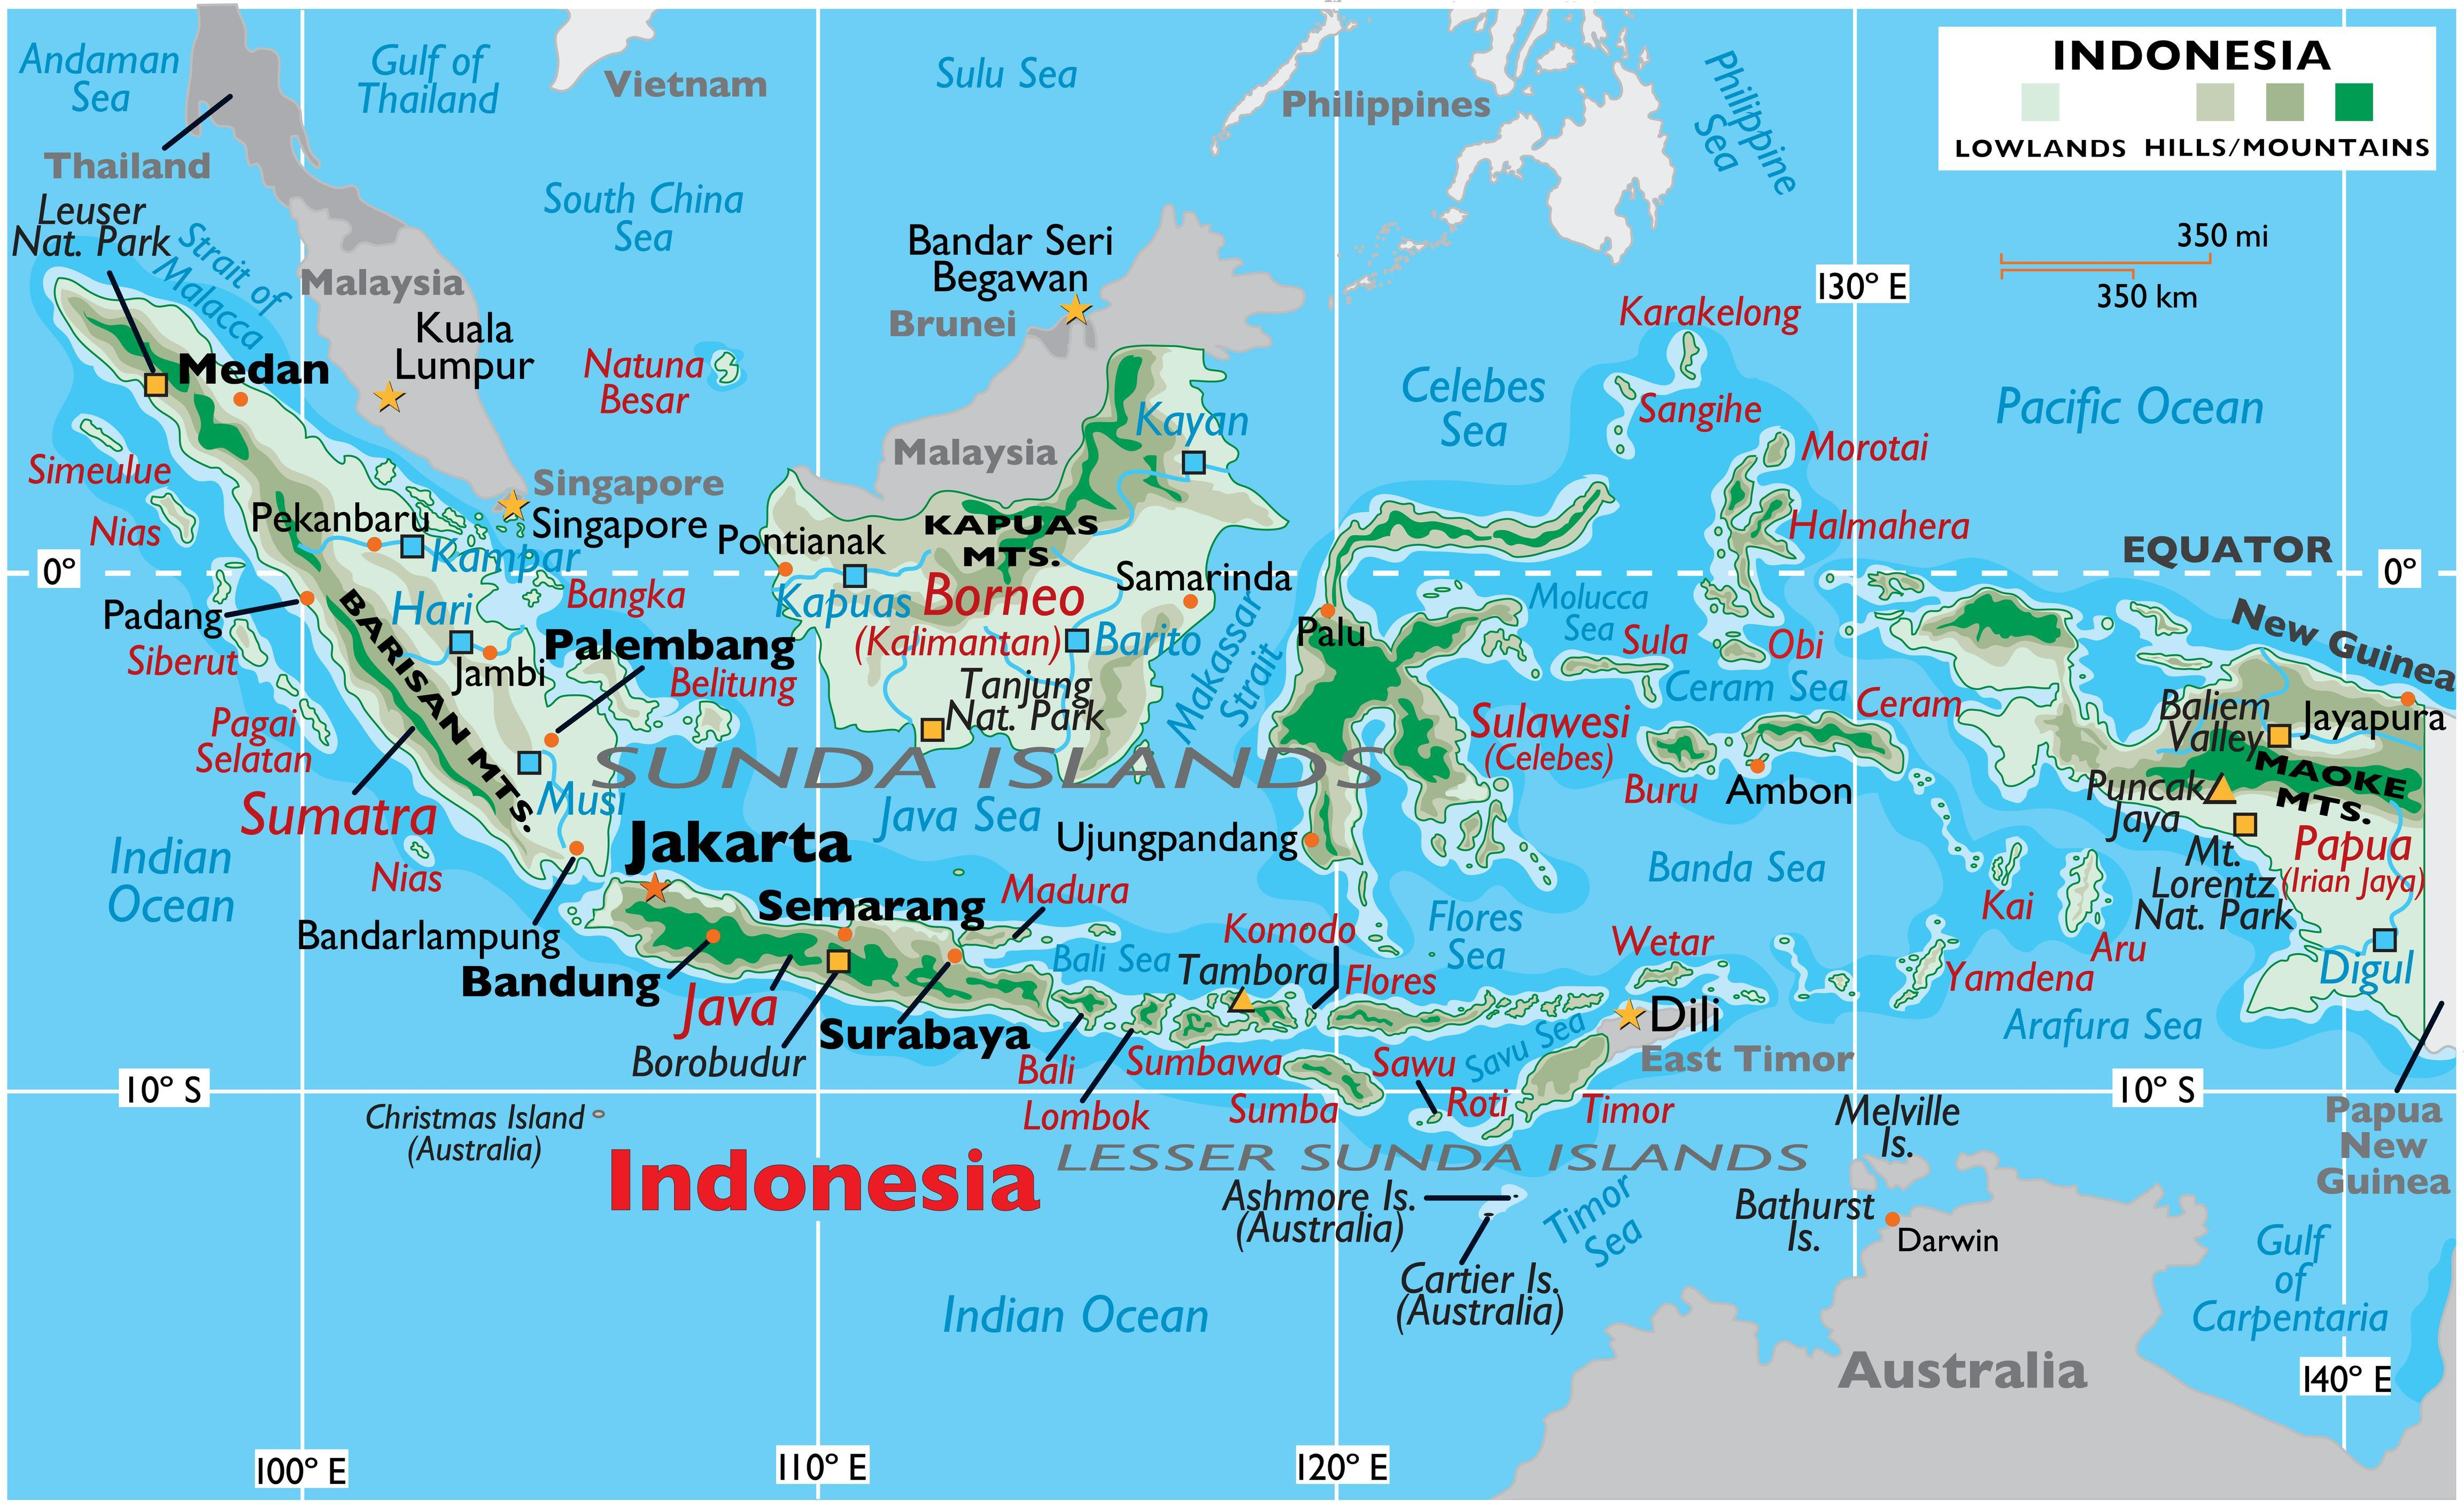
\includegraphics[width=\linewidth]{indonesia-map.eps}
    \caption{インドネシアの地図}\label{indonesiamap}
  \end{figure}
  \subsection{地理}
  前に説明した通り, インドネシアはシンガポール, マレーシア, オーストラリアの間にあり, 面積は約$190.000 km^2$で, インドネシアは世界で14番目に大きな国土面積を持っています. インドネシアは多数の島々を有することで知られており, 周囲を海に囲まれ, 17,508以上の島が存在します\cite{ANDREFOUET2022104848}. 図\ref{indonesiamap}を見ると, インドネシアにはスマトラ島, ジャワ島, カリマンタン島, スラウェシ島, そしてパプア島という本島があります. 各島には全く異なる文化や言語が存在します.\\
  \subsection{人口と民族}
  2020年の国勢調査によると, インドネシアの人口は約2億7,000万人で, 世界で4番目に多いです\cite{unstats2023}. その地理的条件と歴史的背景から, インドネシアには1,331以上の公的に認定された民族集団が存在し, 700以上の言語が国全体にわたって分布しています.\\
  \begin{figure}
    \centering
    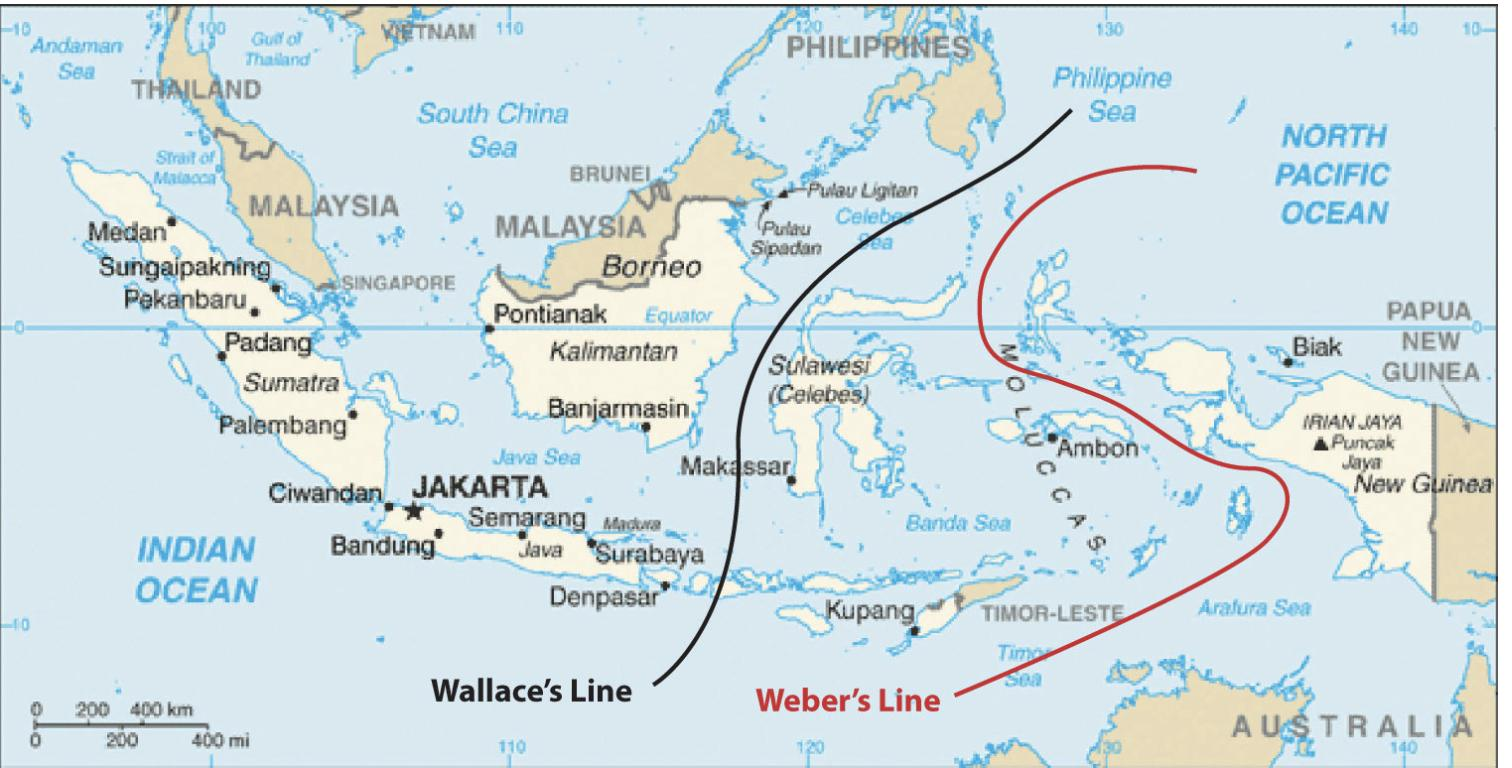
\includegraphics[width=\linewidth]{webber-wallace-line.eps}
    \caption{ウォレスとウェーバーの路線地図}\label{wallaceweber}
  \end{figure}
  \subsection{博物}
  また, 民族だけでなく, インドネシアの動植物も非常に興味深いと思います. 図\ref{wallaceweber}を参考にすると, 1800年代のイギリスの博物学者アルフレッド・ラッセル・ウォレスはインドネシアの列島の中央に線を引き, 動植物の種類を明確に区別しました. ほとんどの動物の種, 特に鳥類は, その線を越えない傾向があります. その線の左側には, アジアでも見られる動物が含まれています. 一方, 右側には, オーストラリアでも見られる動物が含まれています. この線によって分けられているため, インドネシアは豊かな生物多様性を持っています\cite{wallaceline}
  \subsection{宗教}
  インドネシアは歴史的にシャーマニズムの国でしたが、インドの商人たちが岸に到達し、地元の人々にヒンドゥー教を教えたことで変わりました。ヒンドゥー教がその時期に広まり、ヒンドゥー教の名のもとに新しい王国が興亡を繰り返しました。その後、仏教がインドネシアの商人たちによって伝わり、当時最も新しく人気のある宗教となりました。それも、アラビアの商人を通じてイスラム教がシルクロードを経て伝わるまでのことです。イスラム教はインドネシアで急速に広まり、現在もその影響は続いています。現在、インドネシアの人口の87%がイスラム教徒であり、残りはキリスト教、カトリック、儒教、ヒンドゥー教、仏教が信仰されています。大多数がムスリムであるにもかかわらず、インドネシアは憲法に基づいて宗教の自由を保障しているため、厳密にはムスリム国家ではありません。
  \section{歴史}


  \bibliographystyle{plain}
  \bibliography{citations}
\end{document}